\section{Introduction}

\begin{frame}{Motivation: multiphase flow simulation methods}
    \framesubtitle{Lagrangian / Eulerian Interface Advection (LEIA) methods}

    \begin{center}
    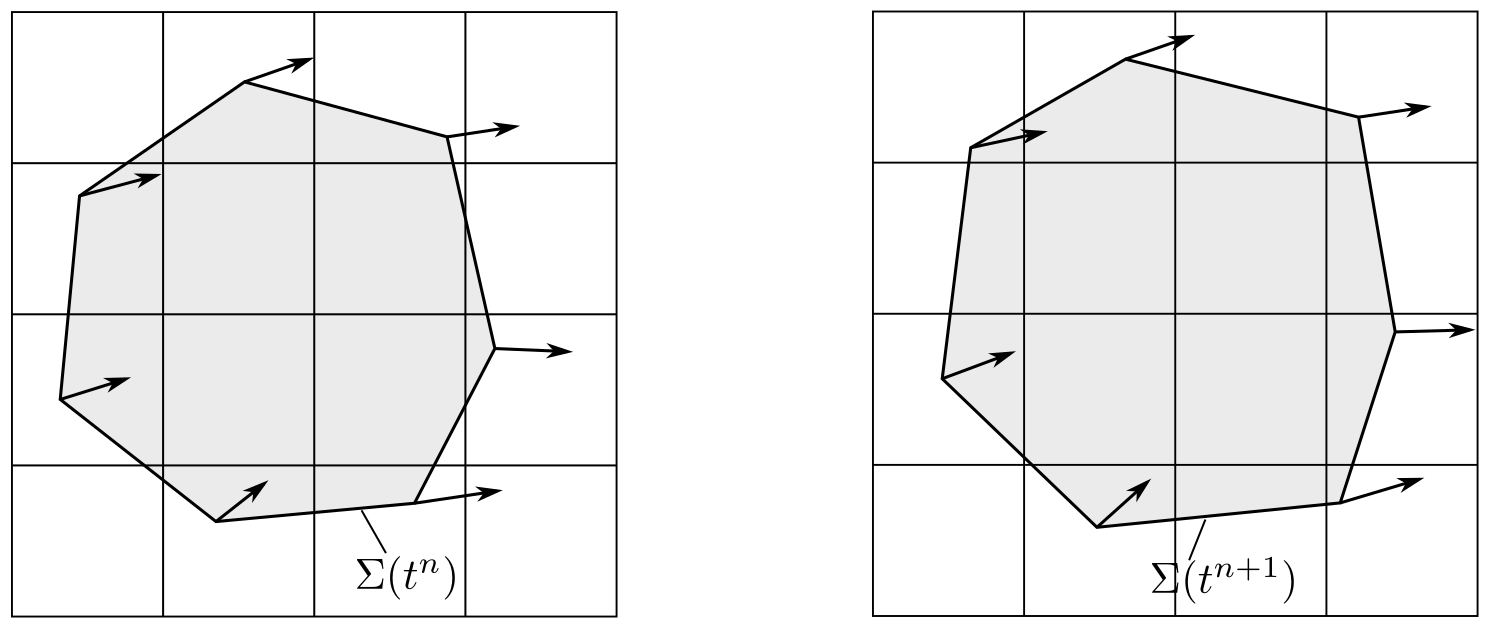
\includegraphics[width=0.7\textwidth]{figures/interface.png}
    \end{center}
    \begin{itemize}
        \item Fluids that do not mix are separated by an interface $\Sigma(t)$ (surface in 3D). 
        \item Goal: track $\Sigma(t)$ as it moves in time $t$ and changes its topology. 
    \end{itemize}

\end{frame}

\begin{frame}{Motivation: multiphase flow simulation software}
    \framesubtitle{Lagrangian / Eulerian Interface Advection (LEIA) Methods}

    \vfill
    LEIA methods
    \footnote{Marić, T., Marschall, H., \& Bothe, D. (2015). lentFoam–A hybrid Level Set/Front Tracking method on unstructured meshes. Computers \& Fluids, 113, 20-31.}\textsuperscript{,}
    \footnote{\footnotesize Tolle, T., Bothe, D., \& Marić, T. (2020). SAAMPLE: A Segregated Accuracy-driven Algorithm for Multiphase Pressure-Linked Equations. Computers \& Fluids, 200, 104450.}\textsuperscript{,}
    \footnote{Marić, T., Kothe, D. B., \& Bothe, D. (2020). Unstructured un-split geometrical Volume-of-Fluid methods–A review. Journal of Computational Physics, 420, 109695.}\textsuperscript{,}
    \footnote{\footnotesize Marić, T. (2021). Iterative Volume-of-Fluid interface positioning in general polyhedrons with Consecutive Cubic Spline interpolation. Journal of Computational Physics: X, 11, 100093.}\textsuperscript{,}
    \footnote{\footnotesize Tolle, T., Gründing, D., Bothe, D., \& Marić, T. (2021). Computing volume fractions and signed distances from triangulated surfaces immersed in unstructured meshes. arXiv preprint arXiv:2101.08511.}
    require \textbf{thorough testing}: 
    \begin{itemize}
        \item \textbf{Verification} cases: evolution of $\Sigma(t)$ and two-phase flows with exact solutions. 

        \item \textbf{Validation} with respect to experiments.  

        \item Testing \textbf{serial and parallel computational efficiency}. 
    \end{itemize}

\end{frame}

%\begin{frame}{Motivation: Level Set / Front Tracking method\footnote{\footnotesize Marić, T., Marschall, H., \& Bothe, D. (2015). lentFoam–A hybrid Level Set/Front Tracking method on unstructured meshes. Computers \& Fluids, 113, 20-31.},\footnote{\footnotesize Tolle, T., Bothe, D., \& Marić, T. (2020). SAAMPLE: A Segregated Accuracy-driven Algorithm for Multiphase Pressure-Linked Equations. Computers \& Fluids, 200, 104450.}}

    %\vfill
    %\begin{center}
        %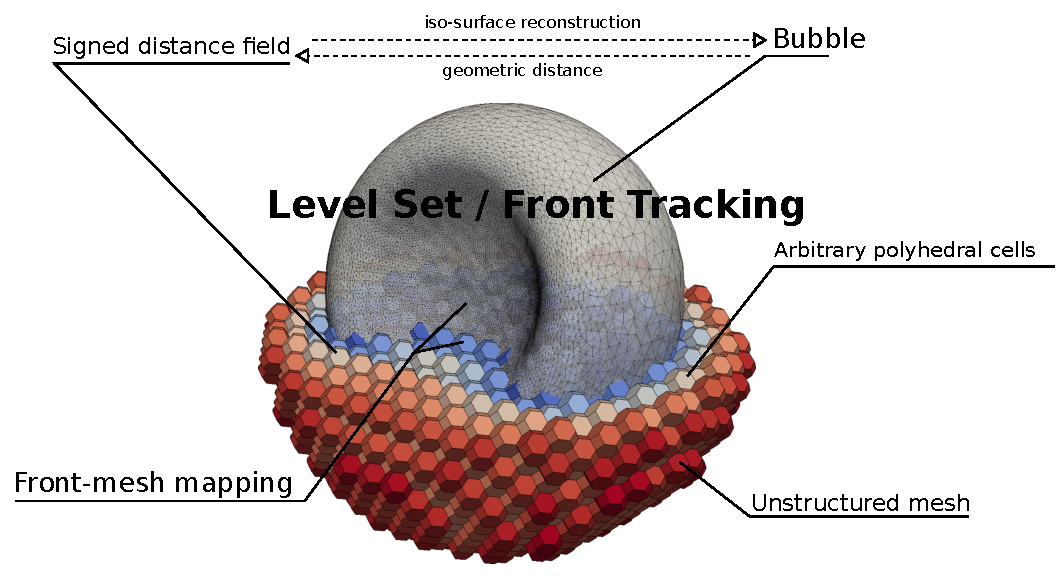
\includegraphics[width=0.5\textwidth]{figures/lent-schematic.pdf}
    %\end{center}
%\end{frame}

%\begin{frame}{Motivation: geometrical un-split Volume-of-Fluid method\footnote{Marić, T., Kothe, D. B., \& Bothe, D. (2020). Unstructured un-split geometrical Volume-of-Fluid methods–A review. Journal of Computational Physics, 420, 109695.}}

    %\vfill
    %\begin{center}
        %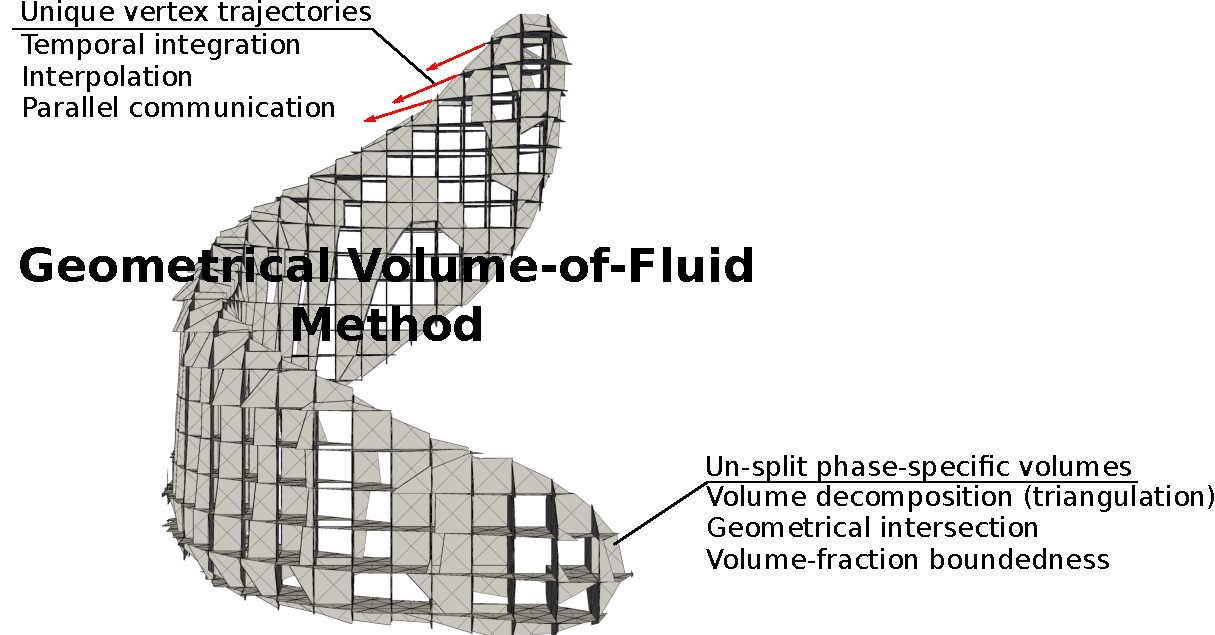
\includegraphics[width=0.6\textwidth]{figures/geovof-schematic.pdf}
    %\end{center}
%\end{frame}

\begin{frame}{Computational Science and Engineering software in\\university research groups}
	\framesubtitle{Boundary and initial conditions}
	
	\vfill
	\begin{itemize}
            \item Publish or perish \faGraduationCap\footnote{Symbol of a publish-or-perish simplification of the workflow :)} prioritizes publications over scientific software.
		\item Dedicated resources for increasing software quality are usually not available.
		\item Ph.D. students rotate every ~3-5 years, postdocs every 1-2 years. 
			\begin{itemize}
				\item Little or no overlap between successors and predecessors. 
			\end{itemize}
		\item Large-scale software design is not a necessary part of the CSE curriculum. 
			\begin{itemize}
				\item Different CSE background: (Applied) Mathematics, Mechanical Engineering, Physics, Informatics.
			\end{itemize}
		\item Real-world example: onboarding people into \href{https://www.openfoam.com/documentation/guides/latest/api/classes.html}{\beamergotobutton{OpenFOAM}} module development.
	\end{itemize}
\end{frame}

\begin{frame}{NFDI4Ing to the rescue!}
\framesubtitle{Resources for engineering research software}
    \vfill

    \begin{center}
    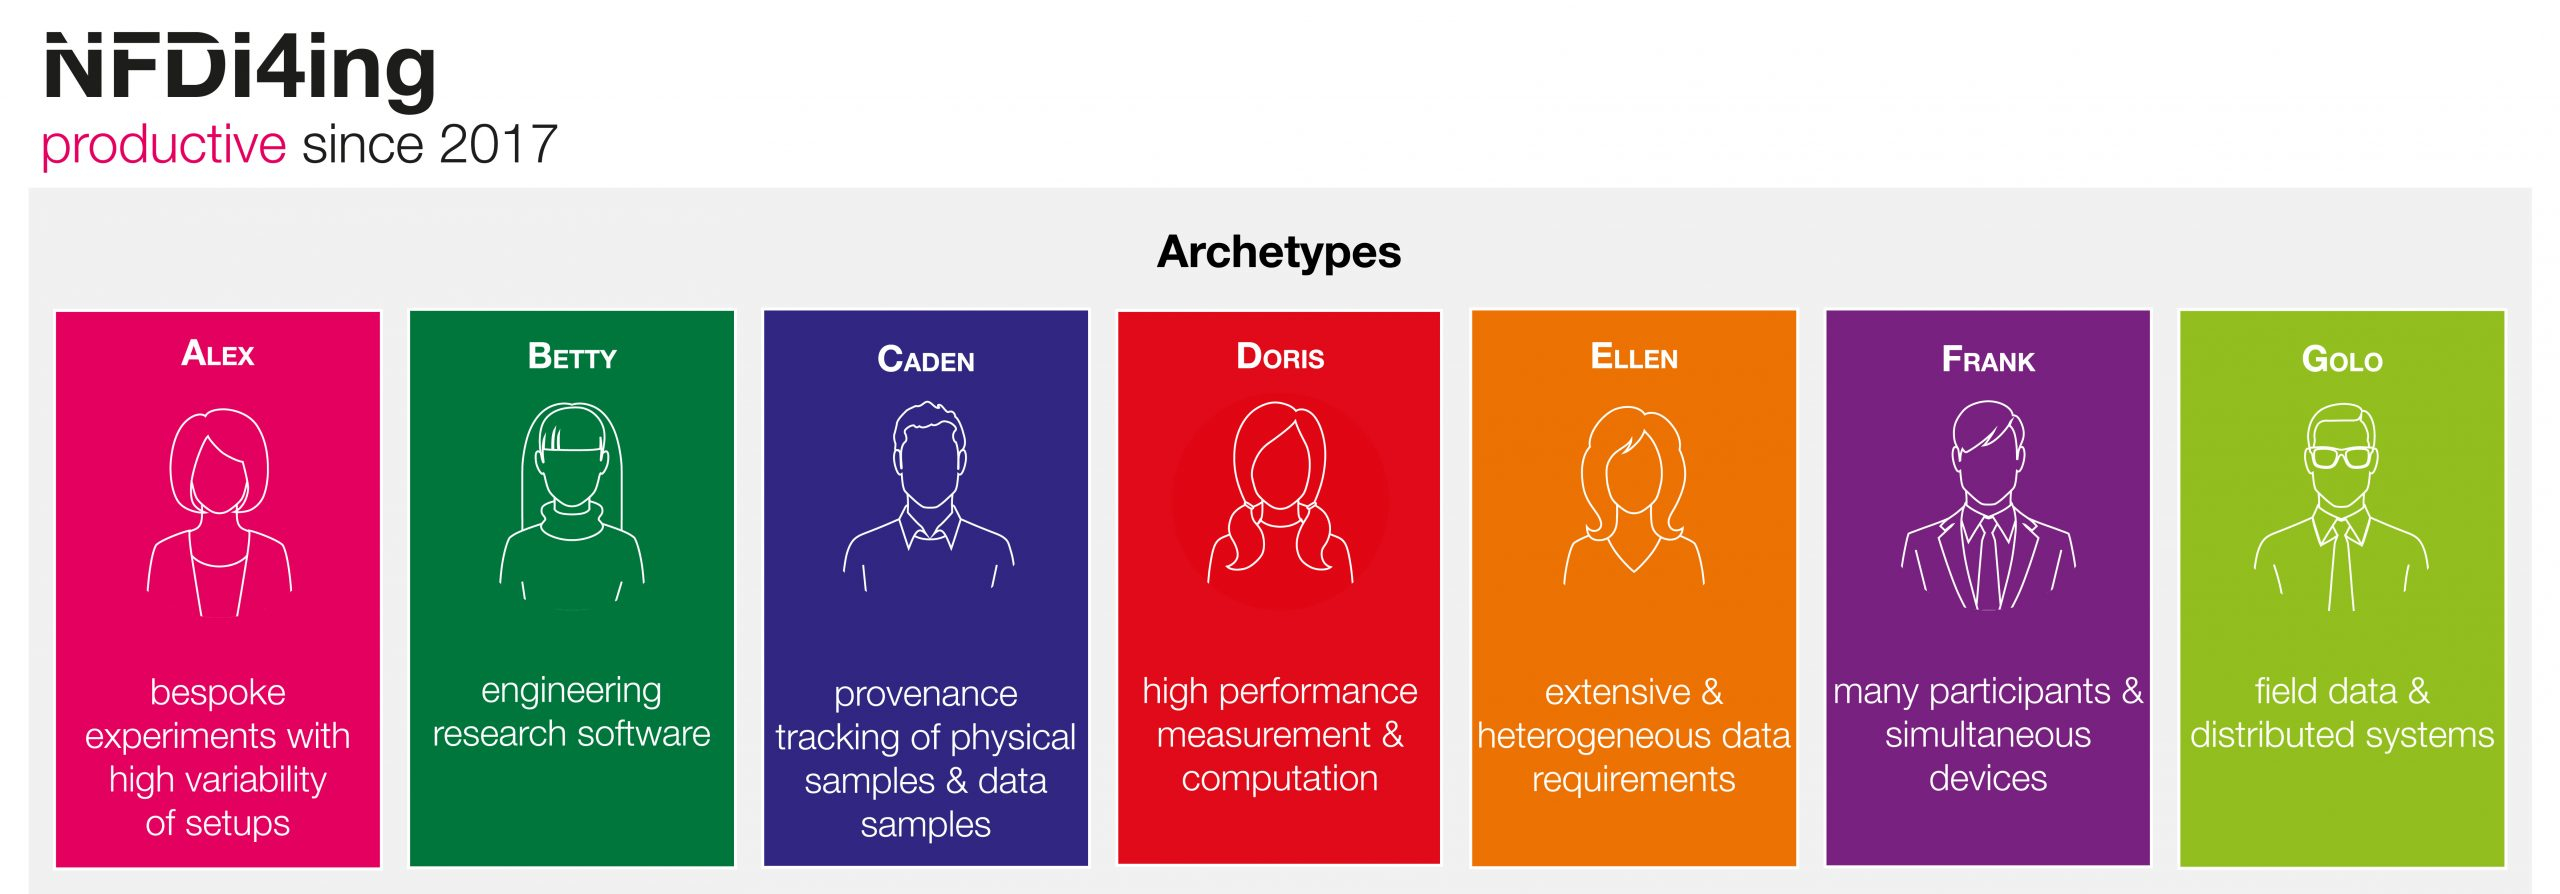
\includegraphics[width=\textwidth]{figures/nfdi4ing.jpg}
    \end{center}
    \href{https://nfdi4ing.de}{NFDI4Ing} resources. 

\end{frame}

\begin{frame}{BSSW to the rescue!}
\framesubtitle{Resources for engineering research software}
    \vfill

    \begin{center}
    
\includegraphics[width=0.6\textwidth]{figures/bssw.png}
    \end{center}
    \href{https://bssw.io}{Better Scientific Software} resources. 

\end{frame}


\begin{frame}{Computational Science and Engineering software in\\university research groups}
    \framesubtitle{The chaos scientific legacy code}
        \vfill
	
    \begin{columns}
        \begin{column}[c]{0.2\textwidth}
            \begin{center}
            
\includegraphics[width=\textwidth]{figures/betty.jpg}
            \end{center}
        \end{column}
        \begin{column}[c]{0.8\textwidth}
            Betty is a CSE researcher, working with a legacy research code.\\
            Why is Betty so (rightfully) angry? 
            \begin{itemize}
                \item Betty inherited a \textbf{research software that is only partially tested}.
                \item Betty inherited a \textbf{research software that isn't automatically tested}.
                    \begin{itemize}
                        \item Betty changes one part of the code and gets her model running, only to see 10 other things fail, after days of manually running tests. 
                    \end{itemize}
                \item Betty's software has \textbf{no documentation of the scientific workflow}. 
                    \begin{itemize}
                        \item Betty doesn't know how to use existing scripts to run simulations and analyze (reproduce) results. 
                    \end{itemize}
                \item Betty's software has \textbf{disjoint (diverging) versions} - that she can't integrate. 
                \item \textbf{Betty can't even find code versions used to generate results in the publications from her research group.} 
            \end{itemize}
        \end{column}
    \end{columns}

\end{frame}

\begin{frame}{Computational Science and Engineering software in\\university research groups}
    \framesubtitle{The chaos of developing entirely new research software}
    \vfill

    \epigraph{"Après moi, le déluge" - "After me, the flood"}{\href{https://en.wikipedia.org/wiki/Apr\%C3\%A8s_moi,_le_d\%C3\%A9luge}{Louis XV of France}}

    Research software generally does not matter, as long as papers are published (\faGraduationCap).
    
    \medskip

    \textbf{Missed opportunities}
    \begin{itemize}
        \item \emph{Finding results} made easy by cross-linking code versions, data and publications. 
        \item \emph{Faster extension / combination of existing ideas} if their respective versions are integrated. 
        \item \emph{Faster comparison of results} with previous ideas automating verification / validation. 
        \item \emph{Automatic reproducibility} of results using automated testing and version control. 
        \item \emph{Faster onboarding} with documented scientific verification and validation workflows. 
    \end{itemize}

\end{frame}

\begin{frame}{Computational Science and Engineering software in\\university research groups}
    \framesubtitle{Continuous integration and cross-linking to the rescue}
    \vfill

    \textbf{Automated testing} (verification and validation), \textbf{version control}, and \textbf{cross-linking} reports, source code and research data increase Findability, Accessibility and Reproducibility (\href{ https://www.go-fair.org/fair-principles}{FAIR}) and \textbf{speed up research.} 

    \begin{itemize}

        \item \textbf{Continuous Integration (CI) = automatic testing + version control.}

        \item CSE research requires \textbf{scientific workflows}: initialize simulations, run parameter variations, agglomerate data, visualize, and check results.  
        \item CI can be used to \textbf{automate and document scientific workflows}. 
        \item CI ensures that the \textbf{integration of new changes does not break existing functionality}.
        \item Once the changes are integrated, the publication, the source code and the data are published on pre-print and data repositories and \textbf{cross-linked} git tags and DOIs. 
    \end{itemize}

\end{frame}

